\documentclass{standalone}

\usepackage[dvipsnames]{xcolor}
\usepackage{tikz}

\usepackage{booktabs}

\usepackage{fontspec}
\setmainfont{Tex Gyre Schola}

\usepackage{array}
%\renewcommand{\arraystretch}{2}
\begin{document}

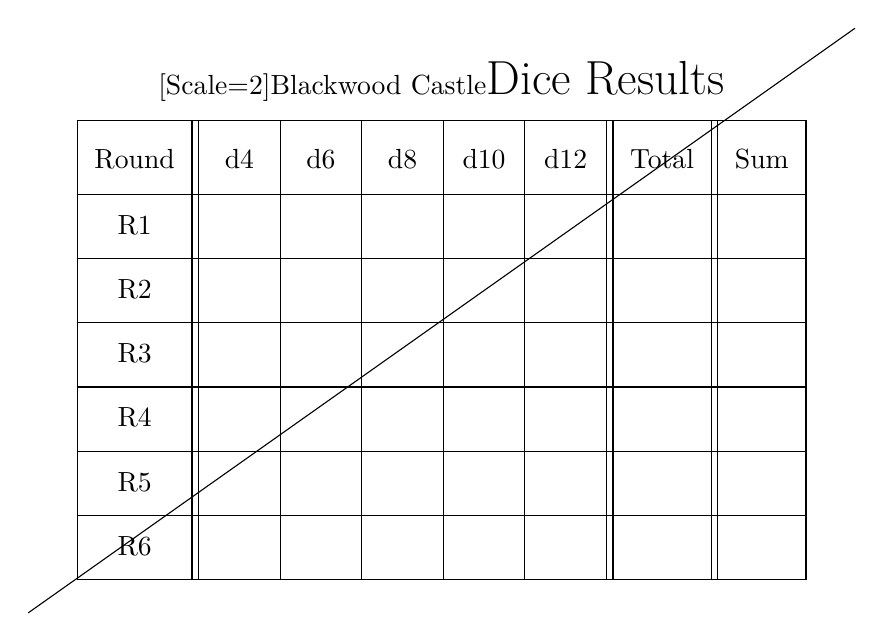
\begin{tikzpicture}

%\path[draw] (-52.5mm,-74.25mm) -- (52.5mm, 74.25mm);
\path[draw] (-52.5mm, -37.125mm) -- (52.5mm, 37.125mm);

\node at (0,0) {
\begin{tabular}{|c||m{6mm}|m{6mm}|m{6mm}|m{6mm}|m{6mm}||c||c|}%||rrrrrl|l|}
\multicolumn{8}{c}{\setmainfont[Scale=2]{Blackwood Castle}\LARGE Dice Results} \\[2mm]\hline
Round\raisebox{-3mm}{\rule{0mm}{9mm}} & \centering d4 & \centering d6 & \centering d8 & \centering d10 & \centering d12 & Total & Sum\\[2mm]\hline % & 2 & 3 & 5 & 7 & 11 & Bonus & Total \\\hline
R1\raisebox{-3mm}{\rule{0mm}{8mm}} & & & & & & & \\\hline%% & & & & & & &\\
R2\raisebox{-3mm}{\rule{0mm}{8mm}} & & & & & & & \\\hline
R3\raisebox{-3mm}{\rule{0mm}{8mm}} & & & & & & & \\\hline
R4\raisebox{-3mm}{\rule{0mm}{8mm}} & & & & & & & \\\hline
R5\raisebox{-3mm}{\rule{0mm}{8mm}} & & & & & & & \\\hline
R6\raisebox{-3mm}{\rule{0mm}{8mm}} & & & & & & & \\\hline
%R7\raisebox{-3mm}{\rule{0mm}{8mm}} & & & & & & \\\hline
%R8\raisebox{-3mm}{\rule{0mm}{8mm}} & & & & & & \\\hline
%R9\raisebox{-3mm}{\rule{0mm}{8mm}} & & & & & & \\\hline
%\phantom{0}R10\raisebox{-3mm}{\rule{0mm}{8mm}} & & & & & & \\\hline
%\phantom{1}R11\raisebox{-3mm}{\rule{0mm}{8mm}} & & & & & & \\\hline
%\phantom{2}R12\raisebox{-3mm}{\rule{0mm}{8mm}} & & & & & & \\\hline
%\phantom{3}R13\raisebox{-3mm}{\rule{0mm}{8mm}} & & & & & & \\\hline
%\phantom{4}R14\raisebox{-3mm}{\rule{0mm}{8mm}} & & & & & & \\

\end{tabular}
};
\end{tikzpicture}
\end{document}